% ============================================================
%  يُترجَم بـ XeLaTeX  (في Overleaf: Menu → Compiler → XeLaTeX)
%  الخط: Amiri (متوفر في Overleaf، أو حمّله من github.com/aliftype/amiri)
% ============================================================
\documentclass[12pt,a4paper]{article}
\usepackage[a4paper,margin=1.2cm,top=2.3cm,bottom=2.9cm,headheight=15pt,footskip=1.5cm]{geometry}
\usepackage{amsmath,amssymb}
\usepackage{icomma}
\usepackage[english,bidi=default,layout=lists]{babel}
\babelprovide[import,main]{arabic}
\babelfont{rm}[Scale=1.08]{Amiri}
\babelfont{sf}[Scale=1.08]{Amiri}
\usepackage[most]{tcolorbox}
\usepackage{tikz}
\usetikzlibrary{arrows.meta,calc,shadings}
\usepackage{array}
\usepackage{colortbl}
\usepackage{fancyhdr}
\usepackage{titlesec}
\usepackage{enumitem}
\usepackage{collcell}
\usepackage{needspace}
\usepackage{etoolbox}
\newcolumntype{C}{>{\collectcell\ar}c<{\endcollectcell}}
\pretocmd{\section}{\Needspace{15\baselineskip}}{}{}
\pretocmd{\subsection}{\Needspace{11\baselineskip}}{}{}

\definecolor{cDef}{HTML}{1F4E9C}
\definecolor{cThm}{HTML}{B3261E}
\definecolor{cRem}{HTML}{2E7D32}
\definecolor{cEx}{HTML}{C76B00}
\definecolor{cMeth}{HTML}{6A1B9A}
\definecolor{cSol}{HTML}{00695C}
\definecolor{cSec}{HTML}{1F3A68}

\titleformat{\section}{\Large\bfseries\color{cSec}}{\thesection.}{0.6em}{}[{\color{cSec!60}\titlerule[1pt]}]
\titleformat{\subsection}{\large\bfseries\color{cThm!85!black}}{\thesubsection.}{0.5em}{}
\titlespacing*{\section}{0pt}{14pt}{8pt}
\titlespacing*{\subsection}{0pt}{10pt}{5pt}
\setlength{\parindent}{0pt}
\setlength{\parskip}{4pt}
\setlist{itemsep=2pt,topsep=3pt}

\newtcolorbox{arbox}[3][]{enhanced,
  colback=#2!5,colframe=#2!80!black,arc=2mm,boxrule=0.8pt,
  left=6pt,right=6pt,top=8pt,bottom=5pt,
  fonttitle=\bfseries,coltitle=white,
  title={\foreignlanguage{arabic}{#3}},
  attach boxed title to top right={xshift=-5mm,yshift=-3mm},
  boxed title style={colback=#2!80!black,arc=1.5mm,boxrule=0pt},
  before upper={\selectlanguage{arabic}},
  before skip=8pt,after skip=8pt,breakable,#1}
\newenvironment{BOX}[2]{\begin{otherlanguage}{english}\begin{arbox}{#1}{#2}}{\end{arbox}\end{otherlanguage}}
\newenvironment{tarif}[1][تعريف]{\begin{BOX}{cDef}{#1}}{\end{BOX}}
\newenvironment{khassia}[1][خاصية]{\begin{BOX}{cThm}{#1}}{\end{BOX}}
\newenvironment{molahada}[1][ملاحظة]{\begin{BOX}{cRem}{#1}}{\end{BOX}}
\newenvironment{mithal}[1][مثال]{\begin{BOX}{cEx}{#1}}{\end{BOX}}
\newenvironment{tariqa}[1][طريقة]{\begin{BOX}{cMeth}{#1}}{\end{BOX}}

\newcounter{exo}
\newenvironment{tamrin}[1]{\stepcounter{exo}\begin{BOX}{cSec}{التمرين \theexo: #1}}{\end{BOX}}
\newenvironment{hal}{\Needspace{12\baselineskip}\begin{otherlanguage}{english}\begin{arbox}[breakable]{cSol}{حل التمرين \theexo}}{\end{arbox}\end{otherlanguage}}

\newenvironment{LTR}{\begin{otherlanguage}{english}}{\end{otherlanguage}}
\newcommand{\ar}[1]{\foreignlanguage{arabic}{#1}}

\renewcommand{\dots}{\mathinner{\ldotp\ldotp\ldotp}}
\renewcommand{\ldots}{\mathinner{\ldotp\ldotp\ldotp}}
\renewcommand{\cdots}{\mathinner{\cdotp\cdotp\cdotp}}
\newcommand{\N}{\mathbb{N}}
\newcommand{\Z}{\mathbb{Z}}
\newcommand{\D}{\mathbb{D}}
\newcommand{\Q}{\mathbb{Q}}
\newcommand{\R}{\mathbb{R}}
\newcommand{\pgcd}{\operatorname{PGCD}}
\newcommand{\ppcm}{\operatorname{PPCM}}

% \NLseg{a}{b}{[}{]} ; \NLright{a}{[} ; \NLleft{b}{]}  (interval on a number line)
\newcommand{\NLseg}[4]{\begin{LTR}\begin{tikzpicture}[baseline=-0.6ex]
 \draw[-{Stealth[length=2mm]},gray!70](0,0)--(3.4,0);
 \draw[line width=2pt,cThm!80!black](0.7,0)--(2.7,0);
 \node[cThm!80!black,font=\LARGE] at (0.7,0){$#3$};
 \node[cThm!80!black,font=\LARGE] at (2.7,0){$#4$};
 \node[below=3pt,font=\footnotesize] at (0.7,0){$#1$};
 \node[below=3pt,font=\footnotesize] at (2.7,0){$#2$};
\end{tikzpicture}\end{LTR}}
\newcommand{\NLright}[2]{\begin{LTR}\begin{tikzpicture}[baseline=-0.6ex]
 \draw[-{Stealth[length=2mm]},gray!70](0,0)--(3.4,0);
 \draw[line width=2pt,cThm!80!black](1.3,0)--(3.3,0);
 \node[cThm!80!black,font=\LARGE] at (1.3,0){$#2$};
 \node[below=3pt,font=\footnotesize] at (1.3,0){$#1$};
\end{tikzpicture}\end{LTR}}
\newcommand{\NLleft}[2]{\begin{LTR}\begin{tikzpicture}[baseline=-0.6ex]
 \draw[-{Stealth[length=2mm]},gray!70](0,0)--(3.4,0);
 \draw[line width=2pt,cThm!80!black](0.05,0)--(2.1,0);
 \node[cThm!80!black,font=\LARGE] at (2.1,0){$#2$};
 \node[below=3pt,font=\footnotesize] at (2.1,0){$#1$};
\end{tikzpicture}\end{LTR}}

% ---------- social-media icons (pure TikZ) ----------
\definecolor{cFB}{HTML}{1877F2}
\definecolor{cTG}{HTML}{229ED9}
\definecolor{cIG1}{HTML}{FEDA75}
\definecolor{cIG2}{HTML}{D62976}
\definecolor{cIG3}{HTML}{4F5BD5}
\newcommand{\fbicon}{\begin{LTR}\begin{tikzpicture}[baseline=-0.75ex,x=1em,y=1em]
 \fill[cFB] (0,0) circle (0.55);
 \node[white,inner sep=0,font=\usefont{TU}{lmss}{bx}{n}\small] at (0.04,-0.02) {f};
\end{tikzpicture}\end{LTR}}
\newcommand{\igicon}{\begin{LTR}
\begin{tikzpicture}[baseline=-0.75ex,x=1em,y=1em]
 \shade[lower left=cIG1,lower right=cIG2,upper left=cIG2,upper right=cIG3,rounded corners=0.28em] (-0.55,-0.55) rectangle (0.55,0.55);
 \draw[white,line width=0.09em,rounded corners=0.18em] (-0.36,-0.36) rectangle (0.36,0.36);
 \draw[white,line width=0.09em] (0,0) circle (0.17);
 \fill[white] (0.22,0.22) circle (0.05);
\end{tikzpicture}\end{LTR}}
\newcommand{\tgicon}{\begin{LTR}
\begin{tikzpicture}[baseline=-0.75ex,x=1em,y=1em]
 \fill[cTG] (0,0) circle (0.55);
 \fill[white] (-0.33,0.0) -- (0.32,0.27) -- (0.2,-0.3) -- (0.0,-0.15) -- (-0.08,-0.28) -- (-0.08,-0.08) -- cycle;
 \fill[cTG!70!black] (-0.08,-0.08) -- (0.25,0.2) -- (0.0,-0.15) -- (-0.08,-0.28) -- cycle;
\end{tikzpicture}\end{LTR}}
% page number: black box, white two-digit number, at the right of the social row
\newcommand{\PageBox}{\begin{LTR}\tikz[baseline=(p.base)]\node[fill=black,text=white,inner sep=2.5pt,minimum width=1.6em,minimum height=1.3em,font=\usefont{TU}{lmss}{bx}{n}\small](p){\ifnum\value{page}<10 0\fi\arabic{page}};\end{LTR}}
% visual left-to-right order: Telegram | Instagram | Facebook | page box
\newcommand{\SocialRow}{\begin{otherlanguage}{english}%
 \ar{\textbf{الأستاذ سوايسية هشام للرياضيات}}\ \tgicon\hfill
 \textbf{prof\_hicham\_math}\ \igicon\hfill
 \ar{\textbf{الأستاذ سوايسية هشام للرياضيات}}\ \fbicon\hspace{2.2em}\PageBox\end{otherlanguage}}

\pagestyle{fancy}
\fancyhf{}
\renewcommand{\headrulewidth}{0.6pt}
\renewcommand{\footrulewidth}{0.4pt}
% \SetHeader{right head: document title}{left head: level -- stream}
\newcommand{\SetHeader}[2]{%
 \fancyhead[C]{\parbox{\textwidth}{\ar{#1\hfill #2}}}%
 \fancyfoot[C]{\parbox{\textwidth}{\small\SocialRow}}}
\usepackage{tkz-tab}
\usepackage{multicol}
% variation / sign table (LTR)
\newenvironment{TAB}{\par\begin{center}\begin{LTR}\begin{tikzpicture}[scale=0.95,every node/.style={font=\small}]}{\end{tikzpicture}\end{LTR}\end{center}}
% grid + axes, clipped: \begin{GR}{xmin}{xmax}{ymin}{ymax}{unit cm}
\newenvironment{GR}[5]{\par\begin{center}\begin{LTR}\begin{tikzpicture}[x=#5cm,y=#5cm,font=\footnotesize]
 \draw[gray!25,very thin] (#1,#3) grid (#2,#4);
 \draw[-{Stealth[length=2mm]}] (#1,0)--(#2+0.3,0) node[below left]{$x$};
 \draw[-{Stealth[length=2mm]}] (0,#3)--(0,#4+0.3) node[below left]{$y$};
 \node[below left] at (0,0){$O$};
 \begin{scope}\clip (#1,#3) rectangle (#2,#4);}
{\end{scope}\end{tikzpicture}\end{LTR}\end{center}}
\newcommand{\Ticks}[2]{\foreach \t in {#1} \node[below,font=\scriptsize] at (\t,0){$\t$}; \foreach \t in {#2} \node[left,font=\scriptsize] at (0,\t){$\t$};}
\newcommand{\bx}[1]{\ensuremath{\colorbox{cDef!12}{$\displaystyle #1$}}}
\newcommand{\TwoCol}[4]{\par\begin{LTR}\noindent\begin{minipage}[t]{#1\textwidth}\selectlanguage{arabic}#2\end{minipage}\hfill\begin{minipage}[t]{#3\textwidth}\selectlanguage{arabic}#4\end{minipage}\end{LTR}\par}
\newcommand{\RL}[4]{\TwoCol{#3}{#4}{#1}{#2}}  % \RL{w1}{right content}{w2}{left content}
\newcommand{\ok}{$\textcolor{cRem}{\checkmark}$}
\newcommand{\limn}{\displaystyle\lim_{n\to+\infty}}
% sub-questions, each on its own line
\newenvironment{sq}{\begin{itemize}[leftmargin=2.4em,itemsep=3pt]}{\end{itemize}}
\newcommand{\qa}{\item[(أ)]}\newcommand{\qb}{\item[(ب)]}\newcommand{\qc}{\item[(جـ)]}\newcommand{\qd}{\item[(د)]}\newcommand{\qe}{\item[(هـ)]}
\newcommand{\pa}{\par\smallskip\textbf{(أ)} }\newcommand{\pb}{\par\smallskip\textbf{(ب)} }\newcommand{\pc}{\par\smallskip\textbf{(جـ)} }\newcommand{\pd}{\par\smallskip\textbf{(د)} }\newcommand{\pe}{\par\smallskip\textbf{(هـ)} }
\newcommand{\QQ}[1]{\par\smallskip\textbf{#1.} }
\newenvironment{tmr}{\stepcounter{exo}\begin{BOX}{cSec}{تمرين محلول \theexo}}{\end{BOX}}
\newcommand{\ABC}[3]{\\[2pt]\begin{tabular}{p{0.28\textwidth}p{0.28\textwidth}p{0.28\textwidth}}(جـ) \ #3 & (ب) \ #2 & (أ) \ #1\end{tabular}}
\pretocmd{\section}{\Needspace{24\baselineskip}}{}{}
\newtcbox{\bxtbox}{on line,colback=cDef!12,colframe=cDef!12,boxrule=0pt,arc=1pt,boxsep=0pt,left=2pt,right=2pt,top=1pt,bottom=1pt}
\newcommand{\bxt}[1]{\foreignlanguage{english}{\bxtbox{\ar{#1}}}}
\usepackage{longtable}
\setlength{\LTpre}{4pt}\setlength{\LTpost}{0pt}
\newcommand{\Phase}[1]{\textbf{#1}}
\newcommand{\Fld}[2]{\textbf{#1:}\ #2}
% رأس المذكرة على نمط النموذج: إطار بعنوان «مذكرة رقم»، معلومات الحصة، ثم إطار الكفاءات
\newcommand{\ModhHead}[9]{%
\begin{LTR}
\begin{tcolorbox}[enhanced,colback=white,colframe=cThm!85!black,arc=4mm,boxrule=1pt,top=14pt,bottom=6pt,left=8pt,right=8pt,
 overlay={\node[fill=cThm!85!black,text=white,rounded corners=3mm,inner xsep=14pt,inner ysep=4pt,font=\large\bfseries] at ([yshift=0pt]frame.north){\ar{مذكرة رقم #1}};},
 before upper={\selectlanguage{arabic}}]
\begin{tabular}{@{}p{0.4\linewidth}p{0.55\linewidth}@{}}
\Fld{المستوى}{#2} & \Fld{الثانوية}{\dotfill}\\[3pt]
\Fld{المادة}{رياضيات} & \Fld{ميدان التعلم}{#3}\\[3pt]
\Fld{المدة}{#5} & \Fld{الوحدة التعلمية}{#4}\\[3pt]
\Fld{الأستاذ}{\dotfill} & \Fld{المحتوى المعرفي}{#6}\\
\end{tabular}
\end{tcolorbox}
\begin{tcolorbox}[enhanced,colback=white,colframe=cThm!85!black,arc=3mm,boxrule=0.8pt,sidebyside,sidebyside align=top,lefthand ratio=0.5,
 segmentation style={dashed,cThm!60},before upper={\selectlanguage{arabic}},before lower={\selectlanguage{arabic}}]
\textbf{الكفاءات المستهدفة:}\par #8
\tcblower
\textbf{الكفاءات القبلية:}\par #7
\end{tcolorbox}
\end{LTR}
\par\smallskip\textbf{الوسائل:} #9\par\smallskip}
\newenvironment{Sayr}{%
\begin{LTR}\renewcommand{\arraystretch}{1.25}\setlength{\tabcolsep}{4pt}\relpenalty=10000\binoppenalty=10000\tolerance=9000\emergencystretch=0.3\linewidth
\begin{longtable}{|p{0.09\textwidth}|>{\centering\arraybackslash}p{0.05\textwidth}|p{0.71\textwidth}|>{\centering\arraybackslash}p{0.09\textwidth}|}
\hline\rowcolor{cThm!12}\ar{\footnotesize\textbf{توجيهات وتعاليق}} & \ar{\footnotesize\textbf{المدة}} & \ar{\textbf{سير الحصة}} & \ar{\footnotesize\textbf{مراحل الحصة}}\\\hline\endhead
\hline\endfoot}{\end{longtable}\end{LTR}}
% سطر في الجدول: \Row{مرحلة}{سير}{مدة}{توجيهات}
\newcommand{\RaggedEnd}{\leftskip=0pt plus 1fil\relax}
\newcommand{\Row}[4]{\ar{\small #4} & \ar{#3} & \ar{\RaggedEnd #2} & \cellcolor{cThm!8}\ar{\Phase{#1}}\\\hline}

\newcommand{\Lab}[2]{\foreignlanguage{english}{\tcbox[on line,colback=#1,colframe=#1,boxrule=0pt,arc=2pt,boxsep=1pt,left=5pt,right=5pt,top=1pt,bottom=1pt]{\ar{\textcolor{white}{\textbf{#2}}}}}}
\newcommand{\Num}[1]{\foreignlanguage{english}{\tikz[baseline=(c.base)]\node[fill=cDef,text=white,inner sep=2pt,font=\footnotesize\bfseries](c){#1};}}
\newcommand{\ck}{\ensuremath{{\color{cRem}\checkmark}}}
\newenvironment{Kad}[1]{\par\smallskip\Lab{#1}}{\par}
\newcommand{\RR}[1]{\ifmmode{\color{cThm}#1}\else$\mbox{\color{cThm}#1}$\fi}
\newcommand{\T}[1]{$\mbox{\color{cDef}\bfseries #1}$}
\providecommand{\LW}[1]{{\color{cDef}#1}}
\SetHeader{\small\bfseries\color{cSec}مذكرات محور: الأعداد المركبة والتحويلات النقطية}{\small\color{cSec}السنة الثالثة ثانوي -- علوم تجريبية ، رياضيات ، تقني رياضي}
\begin{document}
\begin{LTR}
\begin{tcolorbox}[enhanced,colback=cThm!85!black,colframe=cThm!85!black,arc=3mm,halign=center,boxrule=0pt,top=12pt,bottom=12pt,before upper={\selectlanguage{arabic}}]
{\color{white}\fontsize{24}{30}\selectfont\bfseries مذكرات محور: الأعداد المركبة والتحويلات النقطية}\\[8pt]
{\color{white}\large السنة الثالثة ثانوي -- علوم تجريبية ، رياضيات ، تقني رياضي}\\[4pt]
{\color{white}\large 12 مذكرة (24 ساعة) -- السنة الدراسية 2026-2027}
\end{tcolorbox}
\end{LTR}
\begin{BOX}{cThm}{يتضمن هذا العمل}
\begin{enumerate}[label=\textbf{مذكرة \arabic{enumi}:},leftmargin=6em,start=67]
\item مجموعة الأعداد المركبة: الشكل الجبري ، التمثيل ، العمليات.
\item مرافق عدد مركب وخواصه.
\item طويلة عدد مركب وتفسيرها الهندسي.
\item المعادلات من الدرجة الثانية في $\mathbb C$ ، الجذران التربيعيان \textbf{(علوم تجريبية)}.
\item عمدة عدد مركب ، الشكل المثلثي.
\item الشكل الأسي ، ترميز أولر ، دستور موافر.
\item توظيف الطويلة والعمدة في الهندسة.
\item الكتابة المركبة للتحويلات: الانسحاب ، التحاكي ، الدوران.
\item حل مسائل هندسية بالتحويلات والأعداد المركبة.
\item التشابه المباشر: تعريف ، كتابته المركبة ، عناصره.
\item التحليل القانوني لتشابه مباشر ، مركب تشابهين.
\item خواص التشابه المباشر وحل مسائل.
\end{enumerate}
الحلول مفصّلة: المعطيات بالأسود ، \T{العناوين} و\RR{النتائج} بلون مختلف ، وكل سؤال في سطر.
\end{BOX}
\newpage
\ModhHead{67}{3 ع ت / 3 ر / 3 ت ر}{أعداد وحساب}{الأعداد المركبة والتحويلات النقطية}{02 سا}{مجموعة الأعداد المركبة: الشكل الجبري ، التمثيل ، العمليات}%
{\begin{itemize}\item الأشعة والمعلم ، المعادلات من الدرجة الثانية في $\mathbb R$.\end{itemize}}%
{\begin{itemize}\item التعرف على الرموز والاصطلاحات ، والتمثيل الهندسي لعدد مركب ، وإجراء العمليات الحسابية.\end{itemize}}%
{المنهاج ، الكتاب المدرسي (الجزء الثاني) ، الآلة الحاسبة ، أدوات الهندسة.}
\begin{Sayr}
\Row{مرحلة الانطلاق}{%
\textbf{التهيئة النفسية:} هل للمعادلة $x^2+1=0$ حلول في $\mathbb R$ ؟}{10 د}{سؤال تاريخي.}
\Row{التشخيص والاكتشاف}{%
\Lab{cEx}{نشاط رقم 01}\ نقبل وجود عدد $i$ حيث $i^2=-1$ ، ونحسب بنفس قواعد $\mathbb R$.\par\textbf{(1)} احسب $i^3$ ، $i^4$ ، $(1+i)^2$.\par\textbf{(2)} انشر $(2+3i)(1-i)$.\par\textbf{(3)} اكتب $\dfrac1{1+i}$ على الشكل $x+iy$.}{35 د}{تمديد الحساب.}
\Row{}{%
\Lab{cDef}{مناقشة النشاط}\par\textbf{(1)} $i^3=i^2\times i=\RR{-i}$ ؛ \quad $i^4=(i^2)^2=\RR{1}$ ؛ \quad $(1+i)^2=1+2i+i^2=\RR{2i}$.\par\textbf{(2)} $(2+3i)(1-i)=2-2i+3i-3i^2=2+i+3=\RR{5+i}$.\par\textbf{(3)} نضرب في $1-i$: $\dfrac{1-i}{(1+i)(1-i)}=\dfrac{1-i}{1-i^2}=\RR{\dfrac12-\dfrac12i}$.}{}{}
\Row{بناء المعارف}{%
\Lab{cDef}{تعريف}\ كل عدد مركب يكتب بطريقة وحيدة $\LW{\RR{z=x+iy}}$ ($\LW{x,y\in\mathbb R}$): $\LW{x=\mathrm{Re}(z)}$ الجزء الحقيقي ، $\LW{y=\mathrm{Im}(z)}$ الجزء التخيلي. $\LW{z}$ حقيقي إذا كان $\LW{y=0}$ ، وتخيلي صرف إذا كان $\LW{x=0}$.}{50 د}{المستوي المركب.}
\Row{}{%
\Lab{cThm}{خاصية}\par\textbf{(1)} $\LW{x+iy=x^{\prime}+iy^{\prime}\iff x=x^{\prime}}$ و $\LW{y=y^{\prime}}$.\par\textbf{(2)} $\LW{i^{4k}=1}$ ، $\LW{i^{4k+1}=i}$ ، $\LW{i^{4k+2}=-1}$ ، $\LW{i^{4k+3}=-i}$.}{}{}
\Row{}{%
\Lab{cDef}{التمثيل الهندسي}\ في معلم متعامد ومتجانس $(O;\vec u,\vec v)$ نرفق بـ $z=x+iy$ النقطة $M(x;y)$ والشعاع $\overrightarrow{OM}$: $z$ \textbf{لاحقة} $M$.\par\smallskip\begin{LTR}\centering 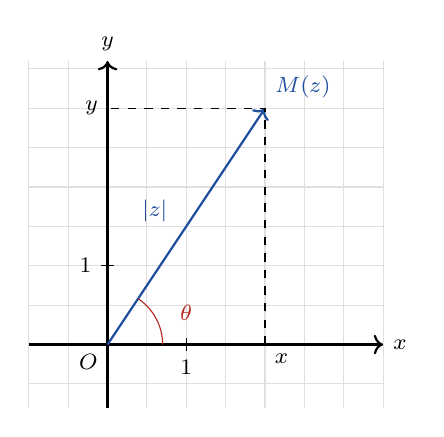
\begin{tikzpicture}[x=1cm,y=1cm,font=\footnotesize]\draw[gray!25,step=0.5] (-1,-0.8) grid (3.5,3.6);\draw[->,thick] (-1,0)--(3.5,0) node[right]{$x$}; \draw[->,thick] (0,-0.8)--(0,3.6) node[above]{$y$};\draw (1,0.08)--(1,-0.08) node[below]{$1$};\draw (0.08,1)--(-0.08,1) node[left]{$1$};\node[below left] at (0,0){$O$};\draw[cDef,thick,->] (0,0)--(2,3) node[above right]{$M(z)$};
\draw[dashed] (2,0)--(2,3)--(0,3); \node[below right] at (2,0){$x$}; \node[left] at (0,3){$y$};
\draw[cThm] (0.7,0) arc (0:56:0.7); \node[cThm] at (1,0.4){$\theta$};
\node[cDef] at (0.6,1.7){$|z|$};\end{tikzpicture}\end{LTR}\par }{}{}
\Row{}{%
\Lab{cEx}{أمثلة محلولة}\par\textbf{(1)} $i^{2026}$: $2026=4\times506+2$ ، إذن $i^{2026}=\RR{-1}$.\par\textbf{(2)} $\dfrac{2+i}{1-i}=\dfrac{(2+i)(1+i)}{2}=\dfrac{2+3i+i^2}2=\RR{\dfrac12+\dfrac32i}$.}{}{}
\Row{}{%
\Lab{cThm!80!black}{حذار}\ لا ترتيب في $\mathbb C$: لا نكتب $z>z^{\prime}$.}{}{}
\Row{التقويم}{%
\Lab{cMeth}{تمرين تطبيقي}\par\textbf{(1)} اكتب على الشكل الجبري: $z=\dfrac{3-i}{1+2i}$.\par\textbf{(2)} عيّن العدد الحقيقي $m$ حتى يكون $(m+i)(1+i)$ تخيليًا صرفًا.}{25 د}{تقويم فردي.}
\Row{}{%
\Lab{cEx}{حل التمرين التطبيقي}\par\textbf{(1)} $z=\dfrac{(3-i)(1-2i)}{1+4}=\dfrac{3-6i-i+2i^2}{5}=\RR{\dfrac15-\dfrac75i}$.\par\textbf{(2)} $(m+i)(1+i)=(m-1)+i(m+1)$: تخيلي صرف إذا كان $m-1=0$ ، أي $\RR{m=1}$.\par\textbf{واجب منزلي:} تمارين من باب الأعداد المركبة.\par\smallskip\textbf{ملاحظات حول سير الحصة:} \dotfill}{}{}
\end{Sayr}
\newpage
\ModhHead{68}{3 ع ت / 3 ر / 3 ت ر}{أعداد وحساب}{الأعداد المركبة والتحويلات النقطية}{02 سا}{مرافق عدد مركب وخواصه}%
{\begin{itemize}\item الشكل الجبري.\end{itemize}}%
{\begin{itemize}\item استعمال خواص المرافق ، وحل معادلات تتضمن $\overline z$.\end{itemize}}%
{المنهاج ، الكتاب المدرسي (الجزء الثاني) ، الآلة الحاسبة ، أدوات الهندسة.}
\begin{Sayr}
\Row{مرحلة الانطلاق}{%
\textbf{التهيئة النفسية:} ما نظيرة النقطة $M(z)$ بالنسبة إلى محور الفواصل؟}{10 د}{سؤال هندسي.}
\Row{التشخيص والاكتشاف}{%
\Lab{cEx}{نشاط رقم 02}\ $z=x+iy$.\par\textbf{(1)} ما لاحقة نظيرة $M(z)$ بالنسبة إلى محور الفواصل؟\par\textbf{(2)} احسب $z+\overline z$ ، $z-\overline z$ ، $z\overline z$ حيث $\overline z=x-iy$.}{35 د}{الخواص في جدول.}
\Row{}{%
\Lab{cDef}{مناقشة النشاط}\par\textbf{(1)} النظيرة $M^{\prime}(x;-y)$ لاحقتها $\RR{x-iy}$: نسميها \textbf{مرافق} $z$.\par\textbf{(2)} $z+\overline z=\RR{2x}$ ؛ \quad $z-\overline z=\RR{2iy}$ ؛ \quad $z\overline z=x^2-(iy)^2=\RR{x^2+y^2}$.}{}{}
\Row{بناء المعارف}{%
\Lab{cDef}{تعريف}\ مرافق $\LW{z=x+iy}$ هو $\LW{\RR{\overline z=x-iy}}$.}{50 د}{المطابقة.}
\Row{}{%
\Lab{cThm}{خاصية}\par\textbf{(1)} $\LW{z+\overline z=2\,\mathrm{Re}(z)}$ ، $\LW{z-\overline z=2i\,\mathrm{Im}(z)}$ ، $\LW{z\overline z=x^2+y^2}$.\par\textbf{(2)} $\LW{\overline{z+z^{\prime}}=\overline z+\overline{z^{\prime}}}$ ، $\LW{\overline{zz^{\prime}}=\overline z\,\overline{z^{\prime}}}$ ، $\LW{\overline{z^n}=\overline z^{\,n}}$ ، $\LW{\overline{\left(\dfrac z{z^{\prime}}\right)}=\dfrac{\overline z}{\overline{z^{\prime}}}}$.\par\textbf{(3)} $\LW{z}$ حقيقي إذا وفقط إذا كان $\LW{z=\overline z}$ ؛ \quad $\LW{z}$ تخيلي صرف إذا وفقط إذا كان $\LW{z=-\overline z}$.}{}{}
\Row{}{%
\Lab{cEx}{أمثلة محلولة}\par\textbf{(1)} حل $2z+i\overline z=3$: نضع $z=x+iy$: $2x+2iy+ix+y=3$.\par\textbf{(2)} $(2x+y)+i(x+2y)=3$: $2x+y=3$ و $x+2y=0$ ، إذن $x=2$ ، $y=-1$: $\RR{z=2-i}$.\par\textbf{(3)} $Z=z^2+\overline z^{\,2}$: $\overline Z=\overline z^{\,2}+z^2=Z$ ، إذن $Z$ \RR{حقيقي}.}{}{}
\Row{}{%
\Lab{cThm!80!black}{حذار}\ في معادلة فيها $z$ و $\overline z$ نضع $z=x+iy$ ونطابق الجزأين الحقيقي والتخيلي.}{}{}
\Row{التقويم}{%
\Lab{cMeth}{تمرين تطبيقي}\par\textbf{(1)} حل في $\mathbb C$: $z+2\overline z=6-i$.}{25 د}{تقويم فردي.}
\Row{}{%
\Lab{cEx}{حل التمرين التطبيقي}\par\textbf{(1)} $x+iy+2x-2iy=3x-iy=6-i$.\par\textbf{(2)} $3x=6$ و $-y=-1$: $\RR{z=2+i}$.\par\textbf{واجب منزلي:} تمارين من باب الأعداد المركبة.\par\smallskip\textbf{ملاحظات حول سير الحصة:} \dotfill}{}{}
\end{Sayr}
\newpage
\ModhHead{69}{3 ع ت / 3 ر / 3 ت ر}{أعداد وحساب}{الأعداد المركبة والتحويلات النقطية}{02 سا}{طويلة عدد مركب وتفسيرها الهندسي}%
{\begin{itemize}\item المرافق ، المسافة في معلم.\end{itemize}}%
{\begin{itemize}\item حساب طويلة عدد مركب ، وتوظيفها في حساب مسافات وتعيين مجموعات نقط.\end{itemize}}%
{المنهاج ، الكتاب المدرسي (الجزء الثاني) ، الآلة الحاسبة ، أدوات الهندسة.}
\begin{Sayr}
\Row{مرحلة الانطلاق}{%
\textbf{التهيئة النفسية:} ما المسافة $OM$ حيث $M(3;4)$ ؟}{10 د}{سؤال.}
\Row{التشخيص والاكتشاف}{%
\Lab{cEx}{نشاط رقم 03}\par\textbf{(1)} احسب $OM$ حيث $M$ لاحقتها $z=3+4i$ ، وقارنها بـ $\sqrt{z\overline z}$.\par\textbf{(2)} $A(z_A)$ و $B(z_B)$: عبّر عن $AB$ بدلالة $z_B-z_A$.}{35 د}{تفسير هندسي.}
\Row{}{%
\Lab{cDef}{مناقشة النشاط}\par\textbf{(1)} $OM=\sqrt{9+16}=\RR{5}$ و $z\overline z=25$: $\RR{OM=\sqrt{z\overline z}}$.\par\textbf{(2)} $\overrightarrow{AB}$ لاحقته $z_B-z_A$: $\RR{AB=|z_B-z_A|}$.}{}{}
\Row{بناء المعارف}{%
\Lab{cDef}{تعريف}\ طويلة $\LW{z=x+iy}$: \par $\LW{\RR{|z|=\sqrt{x^2+y^2}=\sqrt{z\overline z}}}$.}{50 د}{رسم المجموعات.}
\Row{}{%
\Lab{cThm}{خاصية}\par\textbf{(1)} $\LW{|zz^{\prime}|=|z|\,|z^{\prime}|}$ ، $\LW{\left|\dfrac z{z^{\prime}}\right|=\dfrac{|z|}{|z^{\prime}|}}$ ، $\LW{|z^n|=|z|^n}$ ، $\LW{|\overline z|=|z|}$.\par\textbf{(2)} $\LW{\RR{AB=|z_B-z_A|}}$.}{}{}
\Row{}{%
\Lab{cMeth}{مجموعات نقط}\par\textbf{(1)} $\LW{|z-z_A|=r}$ ($\LW{r>0}$): \RR{دائرة} مركزها $\LW{A}$ ونصف قطرها $\LW{r}$.\par\textbf{(2)} $\LW{|z-z_A|=|z-z_B|}$: \RR{محور} القطعة $\LW{[AB]}$.}{}{}
\Row{}{%
\Lab{cEx}{أمثلة محلولة}\par\textbf{(1)} $|1+i\sqrt3|=\sqrt{1+3}=\RR{2}$ ؛ \quad $|(1+i)(3-4i)|=\sqrt2\times5=\RR{5\sqrt2}$.\par\textbf{(2)} $|z-1|=|z+i|$: $AM=BM$ مع $A(1)$ و $B(-i)$: \RR{محور} \RR{القطعة} \RR{$[AB]$}.}{}{}
\Row{}{%
\Lab{cThm!80!black}{حذار}\ \par $|z+z^{\prime}|\neq|z|+|z^{\prime}|$ عمومًا.}{}{}
\Row{التقويم}{%
\Lab{cMeth}{تمرين تطبيقي}\par\textbf{(1)} عيّن مجموعة النقط $M(z)$ حيث $|z-2i|=3$.\par\textbf{(2)} احسب $\left|\dfrac{1+i}{\sqrt3-i}\right|$.}{25 د}{تقويم فردي.}
\Row{}{%
\Lab{cEx}{حل التمرين التطبيقي}\par\textbf{(1)} $AM=3$ مع $A(2i)$: \RR{دائرة} \RR{مركزها} \RR{$A(0;2)$} \RR{ونصف} \RR{قطرها} \RR{$3$}.\par\textbf{(2)} $\dfrac{|1+i|}{|\sqrt3-i|}=\RR{\dfrac{\sqrt2}2}$.\par\textbf{واجب منزلي:} تمارين من باب الأعداد المركبة.\par\smallskip\textbf{ملاحظات حول سير الحصة:} \dotfill}{}{}
\end{Sayr}
\newpage
\ModhHead{70}{3 ع ت / 3 ر / 3 ت ر}{أعداد وحساب}{الأعداد المركبة والتحويلات النقطية}{02 سا}{المعادلات من الدرجة الثانية في $\mathbb C$ ، الجذران التربيعيان}%
{\begin{itemize}\item المميز ، الشكل الجبري ، المرافق.\end{itemize}}%
{\begin{itemize}\item حل معادلات من الدرجة الثانية بمعاملات حقيقية ومعادلات تؤول إليها ، وتعيين الجذرين التربيعيين لعدد مركب (علوم تجريبية).\end{itemize}}%
{المنهاج ، الكتاب المدرسي (الجزء الثاني) ، الآلة الحاسبة ، أدوات الهندسة.}
\begin{Sayr}
\Row{مرحلة الانطلاق}{%
\textbf{التهيئة النفسية:} $z^2-2z+5=0$: $\Delta=-16<0$. هل انتهى الأمر في $\mathbb C$ ؟}{10 د}{سؤال.}
\Row{التشخيص والاكتشاف}{%
\Lab{cEx}{نشاط رقم 04}\par\textbf{(1)} اكتب $-16$ على الشكل $(\delta)^2$ في $\mathbb C$.\par\textbf{(2)} حل $z^2-2z+5=0$ بنفس دساتير $\mathbb R$.}{35 د}{تمديد المميز.}
\Row{}{%
\Lab{cDef}{مناقشة النشاط}\par\textbf{(1)} $-16=16i^2=\RR{(4i)^2}$.\par\textbf{(2)} $z=\dfrac{2\pm4i}2=\RR{1\pm2i}$ (حلان مترافقان).}{}{}
\Row{بناء المعارف}{%
\Lab{cThm}{خاصية}\ $\LW{az^2+bz+c=0}$ ($\LW{a,b,c}$ حقيقية ، $\LW{a\neq0}$) ، $\LW{\Delta=b^2-4ac}$:\par\textbf{(1)} $\LW{\Delta\geqslant0}$: حلول حقيقية كما في $\LW{\mathbb R}$.\par\textbf{(2)} $\LW{\Delta<0}$: حلان مترافقان $\LW{\RR{z=\dfrac{-b\pm i\sqrt{-\Delta}}{2a}}}$.}{50 د}{جذور مترافقة.}
\Row{}{%
\Lab{cEx}{أمثلة محلولة}\par\textbf{(1)} $z^2+z+1=0$: $\Delta=-3$ ، $\RR{z=\dfrac{-1\pm i\sqrt3}2}$.\par\textbf{(2)} $z^3-1=0$: $(z-1)(z^2+z+1)=0$: \par $\RR{z\in\left\{1;\dfrac{-1+i\sqrt3}2;\dfrac{-1-i\sqrt3}2\right\}}$.}{}{}
\Row{}{%
\Lab{cMeth}{الجذران التربيعيان (علوم تجريبية)}\ لـ $\LW{3+4i}$: نبحث عن $\LW{(x+iy)^2=3+4i}$:\par\textbf{(1)} $\LW{x^2-y^2=3}$ ، $\LW{2xy=4}$ ، و $\LW{x^2+y^2=|3+4i|=5}$.\par\textbf{(2)} $\LW{x^2=4}$ ، $\LW{y^2=1}$ ، و $\LW{xy>0}$: الجذران $\LW{\RR{2+i}}$ و $\LW{\RR{-2-i}}$ (تحقق: $\LW{(2+i)^2=3+4i}$ \ck).}{}{}
\Row{}{%
\Lab{cThm!80!black}{حذار}\ لا نكتب $\sqrt{-16}$ ؛ نكتب $-16=(4i)^2$.}{}{}
\Row{التقويم}{%
\Lab{cMeth}{تمرين تطبيقي}\par\textbf{(1)} حل في $\mathbb C$: $z^2-6z+13=0$.\par\textbf{(2)} حل في $\mathbb C$: $(z^2+4)(z^2-2z+2)=0$.}{25 د}{تقويم فردي.}
\Row{}{%
\Lab{cEx}{حل التمرين التطبيقي}\par\textbf{(1)} $\Delta=36-52=-16$: $z=\dfrac{6\pm4i}2=\RR{3\pm2i}$.\par\textbf{(2)} $z^2=-4=(2i)^2$: $z=\pm2i$ ؛ $\Delta=-4$: $z=1\pm i$: \par $\RR{\{2i;-2i;1+i;1-i\}}$.\par\textbf{واجب منزلي:} تمارين من باب الأعداد المركبة.\par\smallskip\textbf{ملاحظات حول سير الحصة:} \dotfill}{}{}
\end{Sayr}
\newpage
\ModhHead{71}{3 ع ت / 3 ر / 3 ت ر}{أعداد وحساب}{الأعداد المركبة والتحويلات النقطية}{02 سا}{عمدة عدد مركب ، الشكل المثلثي}%
{\begin{itemize}\item الطويلة ، الزوايا الموجهة ، الدائرة المثلثية.\end{itemize}}%
{\begin{itemize}\item حساب عمدة عدد مركب غير معدوم ، والانتقال من الشكل الجبري إلى المثلثي والعكس.\end{itemize}}%
{المنهاج ، الكتاب المدرسي (الجزء الثاني) ، الآلة الحاسبة ، أدوات الهندسة.}
\begin{Sayr}
\Row{مرحلة الانطلاق}{%
\textbf{التهيئة النفسية:} ما قيس الزاوية بين $\vec u$ و $\overrightarrow{OM}$ حيث $M(1;1)$ ؟}{10 د}{سؤال.}
\Row{التشخيص والاكتشاف}{%
\Lab{cEx}{نشاط رقم 05}\ $z=1+i$.\par\textbf{(1)} احسب $|z|$.\par\textbf{(2)} احسب $\dfrac{x}{|z|}$ و $\dfrac{y}{|z|}$ ، واستنتج قيسًا $\theta$ للزاوية $(\vec u;\overrightarrow{OM})$.}{35 د}{الدائرة المثلثية.}
\Row{}{%
\Lab{cDef}{مناقشة النشاط}\par\textbf{(1)} $|z|=\RR{\sqrt2}$.\par\textbf{(2)} $\cos\theta=\dfrac1{\sqrt2}=\dfrac{\sqrt2}2$ و $\sin\theta=\dfrac{\sqrt2}2$: $\RR{\theta=\dfrac\pi4}$ ، و \par $z=\sqrt2\left(\cos\dfrac\pi4+i\sin\dfrac\pi4\right)$.}{}{}
\Row{بناء المعارف}{%
\Lab{cDef}{تعريف}\ عمدة $\LW{z\neq0}$: قيس $\LW{\theta}$ للزاوية $\LW{(\vec u;\overrightarrow{OM})}$ ، ونكتب $\LW{\arg z=\theta\ [2\pi]}$. الشكل المثلثي: $\LW{\RR{z=r(\cos\theta+i\sin\theta)}}$ حيث $\LW{r=|z|}$ ، $\LW{\cos\theta=\dfrac xr}$ ، $\LW{\sin\theta=\dfrac yr}$.}{50 د}{الزوايا الشهيرة.}
\Row{}{%
\Lab{cThm}{خاصية}\par\textbf{(1)} $\LW{\arg(zz^{\prime})=\arg z+\arg z^{\prime}}$ ؛ \quad $\LW{\arg\dfrac z{z^{\prime}}=\arg z-\arg z^{\prime}}$ ؛ \quad $\LW{\arg z^n=n\arg z}$.\par\textbf{(2)} $\LW{\arg\overline z=-\arg z}$ ؛ \quad $\LW{\arg(-z)=\arg z+\pi}$ \quad $\LW{[2\pi]}$.}{}{}
\Row{}{%
\Lab{cEx}{أمثلة محلولة}\par\textbf{(1)} $1+i\sqrt3$: $r=2$ ، $\cos\theta=\dfrac12$ ، $\sin\theta=\dfrac{\sqrt3}2$: $\RR{2\left(\cos\dfrac\pi3+i\sin\dfrac\pi3\right)}$.\par\textbf{(2)} $-1+i$: $r=\sqrt2$ ، $\cos\theta=-\dfrac{\sqrt2}2$ ، $\sin\theta=\dfrac{\sqrt2}2$: $\RR{\sqrt2\left(\cos\dfrac{3\pi}4+i\sin\dfrac{3\pi}4\right)}$.}{}{}
\Row{}{%
\Lab{cThm!80!black}{حذار}\ نحدد الربع من إشارتي $\cos\theta$ و $\sin\theta$ معًا ، و $r>0$ دائمًا.}{}{}
\Row{التقويم}{%
\Lab{cMeth}{تمرين تطبيقي}\par\textbf{(1)} اكتب $z=-\sqrt3-i$ على الشكل المثلثي.\par\textbf{(2)} استنتج عمدة لـ $z^2$.}{25 د}{تقويم فردي.}
\Row{}{%
\Lab{cEx}{حل التمرين التطبيقي}\par\textbf{(1)} $r=2$ ، $\cos\theta=-\dfrac{\sqrt3}2$ ، $\sin\theta=-\dfrac12$: $\RR{\theta=-\dfrac{5\pi}6}$.\par\textbf{(2)} $\arg z^2=2\times\left(-\dfrac{5\pi}6\right)=-\dfrac{5\pi}3\equiv\RR{\dfrac\pi3}\ [2\pi]$.\par\textbf{واجب منزلي:} تمارين من باب الأعداد المركبة.\par\smallskip\textbf{ملاحظات حول سير الحصة:} \dotfill}{}{}
\end{Sayr}
\newpage
\ModhHead{72}{3 ع ت / 3 ر / 3 ت ر}{أعداد وحساب}{الأعداد المركبة والتحويلات النقطية}{02 سا}{الشكل الأسي ، ترميز أولر ، دستور موافر}%
{\begin{itemize}\item الشكل المثلثي ، خواص العمدة.\end{itemize}}%
{\begin{itemize}\item الانتقال من الشكل الجبري إلى الأسي والعكس ، واستعمال دستور موافر.\end{itemize}}%
{المنهاج ، الكتاب المدرسي (الجزء الثاني) ، الآلة الحاسبة ، أدوات الهندسة.}
\begin{Sayr}
\Row{مرحلة الانطلاق}{%
\textbf{التهيئة النفسية:} كيف نحسب $(1+i)^8$ بسرعة؟}{10 د}{تحدٍّ.}
\Row{التشخيص والاكتشاف}{%
\Lab{cEx}{نشاط رقم 06}\ نضع $f(\theta)=\cos\theta+i\sin\theta$.\par\textbf{(1)} احسب $f(\theta)\times f(\theta^{\prime})$ وبسّط.\par\textbf{(2)} ماذا تذكرك هذه القاعدة؟}{35 د}{ترميز أولر.}
\Row{}{%
\Lab{cDef}{مناقشة النشاط}\par\textbf{(1)} $f(\theta)f(\theta^{\prime})=\cos\theta\cos\theta^{\prime}-\sin\theta\sin\theta^{\prime}+i(\sin\theta\cos\theta^{\prime}+\cos\theta\sin\theta^{\prime})=\RR{f(\theta+\theta^{\prime})}$.\par\textbf{(2)} نفس قاعدة الأسس $e^ae^b=e^{a+b}$: نكتب $\RR{f(\theta)=e^{i\theta}}$ (ترميز أولر).}{}{}
\Row{بناء المعارف}{%
\Lab{cDef}{تعريف}\ $\LW{e^{i\theta}=\cos\theta+i\sin\theta}$ ؛ الشكل الأسي لـ $\LW{z\neq0}$: $\LW{\RR{z=re^{i\theta}}}$ ($\LW{r=|z|}$ ، $\LW{\theta=\arg z}$).}{50 د}{دستور موافر.}
\Row{}{%
\Lab{cThm}{خاصية}\par\textbf{(1)} $\LW{re^{i\theta}\times r^{\prime}e^{i\theta^{\prime}}=rr^{\prime}e^{i(\theta+\theta^{\prime})}}$ ؛ \quad \par $\LW{\dfrac{re^{i\theta}}{r^{\prime}e^{i\theta^{\prime}}}=\dfrac r{r^{\prime}}e^{i(\theta-\theta^{\prime})}}$.\par\textbf{(2)} $\LW{\left(re^{i\theta}\right)^n=r^ne^{in\theta}}$ ؛ \quad $\LW{\overline{e^{i\theta}}=e^{-i\theta}}$.}{}{}
\Row{}{%
\Lab{cThm}{دستور موافر}\ \par $\LW{\RR{(\cos\theta+i\sin\theta)^n=\cos n\theta+i\sin n\theta}}$.}{}{}
\Row{}{%
\Lab{cEx}{أمثلة محلولة}\par\textbf{(1)} $(1+i)^8=\left(\sqrt2e^{i\frac\pi4}\right)^8=16e^{2i\pi}=\RR{16}$.\par\textbf{(2)} $\dfrac{1+i}{1-i}=\dfrac{\sqrt2e^{i\frac\pi4}}{\sqrt2e^{-i\frac\pi4}}=e^{i\frac\pi2}=\RR{i}$.\par\textbf{(3)} من $(\cos\theta+i\sin\theta)^2=\cos2\theta+i\sin2\theta$: $\RR{\cos2\theta=\cos^2\theta-\sin^2\theta}$ و $\RR{\sin2\theta=2\sin\theta\cos\theta}$.}{}{}
\Row{}{%
\Lab{cThm!80!black}{حذار}\ $r>0$ في الشكل الأسي: \par $-2e^{i\frac\pi3}=2e^{i\frac{4\pi}3}$.}{}{}
\Row{التقويم}{%
\Lab{cMeth}{تمرين تطبيقي}\par\textbf{(1)} احسب $(1+i\sqrt3)^6$.\par\textbf{(2)} اكتب $z=\dfrac{(1+i)^4}{(\sqrt3+i)^2}$ على الشكل الأسي.}{25 د}{تقويم فردي.}
\Row{}{%
\Lab{cEx}{حل التمرين التطبيقي}\par\textbf{(1)} $\left(2e^{i\frac\pi3}\right)^6=64e^{2i\pi}=\RR{64}$.\par\textbf{(2)} $\dfrac{\left(\sqrt2e^{i\frac\pi4}\right)^4}{\left(2e^{i\frac\pi6}\right)^2}=\dfrac{4e^{i\pi}}{4e^{i\frac\pi3}}=\RR{e^{i\frac{2\pi}3}}$.\par\textbf{واجب منزلي:} تمارين من باب الأعداد المركبة.\par\smallskip\textbf{ملاحظات حول سير الحصة:} \dotfill}{}{}
\end{Sayr}
\newpage
\ModhHead{73}{3 ع ت / 3 ر / 3 ت ر}{أعداد وحساب}{الأعداد المركبة والتحويلات النقطية}{02 سا}{توظيف الطويلة والعمدة في الهندسة}%
{\begin{itemize}\item الطويلة والعمدة ، الزوايا الموجهة.\end{itemize}}%
{\begin{itemize}\item التعبير عن خواص أشكال هندسية بالأعداد المركبة ، وتوظيف خواص الطويلة والعمدة لحل مسائل.\end{itemize}}%
{المنهاج ، الكتاب المدرسي (الجزء الثاني) ، الآلة الحاسبة ، أدوات الهندسة.}
\begin{Sayr}
\Row{مرحلة الانطلاق}{%
\textbf{التهيئة النفسية:} كيف نبرهن بالأعداد المركبة أن مثلثًا متقايس الأضلاع؟}{10 د}{سؤال.}
\Row{التشخيص والاكتشاف}{%
\Lab{cEx}{نشاط رقم 07}\ $A$ ، $B$ ، $C$ نقط متمايزة.\par\textbf{(1)} ما طويلة $\dfrac{z_C-z_A}{z_B-z_A}$ ؟\par\textbf{(2)} ما عمدته؟}{35 د}{تفسير النسبة.}
\Row{}{%
\Lab{cDef}{مناقشة النشاط}\par\textbf{(1)} $\left|\dfrac{z_C-z_A}{z_B-z_A}\right|=\RR{\dfrac{AC}{AB}}$.\par\textbf{(2)} $\arg\dfrac{z_C-z_A}{z_B-z_A}=\arg(z_C-z_A)-\arg(z_B-z_A)=\RR{(\overrightarrow{AB};\overrightarrow{AC})}\ [2\pi]$.}{}{}
\Row{بناء المعارف}{%
\Lab{cThm}{خاصية}\ $\LW{\RR{\left|\dfrac{z_C-z_A}{z_B-z_A}\right|=\dfrac{AC}{AB}}}$ و \par $\LW{\RR{\arg\dfrac{z_C-z_A}{z_B-z_A}=(\overrightarrow{AB};\overrightarrow{AC})}\ [2\pi]}$.}{50 د}{جدول الحالات.}
\Row{}{%
\Lab{cMeth}{طبيعة مثلث}\par\textbf{(1)} النسبة $\LW{=e^{\pm i\frac\pi3}}$: مثلث \RR{متقايس} \RR{الأضلاع}.\par\textbf{(2)} النسبة $\LW{=\pm i}$: مثلث \RR{قائم} \RR{ومتساوي} \RR{الساقين} في $\LW{A}$.\par\textbf{(3)} النسبة حقيقية: النقط \RR{على} \RR{استقامة} \RR{واحدة}.\par\textbf{(4)} النسبة تخيلية صرفة: المثلث \RR{قائم} في $\LW{A}$.}{}{}
\Row{}{%
\Lab{cEx}{أمثلة محلولة}\par\textbf{(1)} $A(0)$ ، $B(2)$ ، $C(1+i\sqrt3)$: $\dfrac{z_C-z_A}{z_B-z_A}=\dfrac{1+i\sqrt3}2=e^{i\frac\pi3}$: \RR{متقايس} \RR{الأضلاع}.\par\textbf{(2)} $A(1)$ ، $B(2+i)$ ، $C(4+3i)$: $\dfrac{z_C-z_A}{z_B-z_A}=\dfrac{3+3i}{1+i}=3$ حقيقي: \RR{على} \RR{استقامة} \RR{واحدة}.}{}{}
\Row{}{%
\Lab{cThm!80!black}{حذار}\ ترتيب النقط في النسبة يحدد الزاوية: $\dfrac{z_C-z_A}{z_B-z_A}$ تعطي $(\overrightarrow{AB};\overrightarrow{AC})$.}{}{}
\Row{التقويم}{%
\Lab{cMeth}{تمرين تطبيقي}\par $A(1+i)$ ، $B(3+2i)$ ، $C(3i)$.\par\textbf{(1)} احسب $\dfrac{z_C-z_A}{z_B-z_A}$.\par\textbf{(2)} استنتج طبيعة المثلث $ABC$.}{25 د}{تقويم فردي.}
\Row{}{%
\Lab{cEx}{حل التمرين التطبيقي}\par\textbf{(1)} $\dfrac{-1+2i}{2+i}=\dfrac{(-1+2i)(2-i)}{5}=\dfrac{-2+i+4i+2}{5}=\RR{i}$.\par\textbf{(2)} $AC=AB$ و $(\overrightarrow{AB};\overrightarrow{AC})=\dfrac\pi2$: \RR{قائم} \RR{ومتساوي} \RR{الساقين} \RR{في} \RR{$A$}.\par\textbf{واجب منزلي:} تمارين من باب الأعداد المركبة.\par\smallskip\textbf{ملاحظات حول سير الحصة:} \dotfill}{}{}
\end{Sayr}
\newpage
\ModhHead{74}{3 ع ت / 3 ر / 3 ت ر}{أعداد وحساب}{الأعداد المركبة والتحويلات النقطية}{02 سا}{الكتابة المركبة للتحويلات: الانسحاب ، التحاكي ، الدوران}%
{\begin{itemize}\item التحويلات النقطية (السنة الثانية) ، الشكل الأسي.\end{itemize}}%
{\begin{itemize}\item تعيين الكتابة المركبة لتحويل ، والتعرف على تحويل من كتابته المركبة.\end{itemize}}%
{المنهاج ، الكتاب المدرسي (الجزء الثاني) ، الآلة الحاسبة ، أدوات الهندسة.}
\begin{Sayr}
\Row{مرحلة الانطلاق}{%
\textbf{التهيئة النفسية:} ما الذي يفعله الضرب في $i$ بنقطة من المستوي؟}{10 د}{سؤال.}
\Row{التشخيص والاكتشاف}{%
\Lab{cEx}{نشاط رقم 08}\ $z^{\prime}=iz$.\par\textbf{(1)} قارن $|z^{\prime}|$ و $|z|$.\par\textbf{(2)} قارن $\arg z^{\prime}$ و $\arg z$ ، واستنتج طبيعة التحويل.}{35 د}{تفسير الضرب.}
\Row{}{%
\Lab{cDef}{مناقشة النشاط}\par\textbf{(1)} $|z^{\prime}|=|i||z|=\RR{|z|}$: $OM^{\prime}=OM$.\par\textbf{(2)} $\arg z^{\prime}=\arg z+\dfrac\pi2$: \RR{دوران} \RR{مركزه} \RR{$O$} \RR{وزاويته} \RR{$\frac\pi2$}.}{}{}
\Row{بناء المعارف}{%
\Lab{cThm}{الكتابات المركبة}\par\textbf{(1)} انسحاب شعاعه $\LW{\vec w(b)}$: $\LW{\RR{z^{\prime}=z+b}}$.\par\textbf{(2)} تحاكٍ مركزه $\LW{\Omega(\omega)}$ ونسبته $\LW{k}$: $\LW{\RR{z^{\prime}-\omega=k(z-\omega)}}$.\par\textbf{(3)} دوران مركزه $\LW{\Omega(\omega)}$ وزاويته $\LW{\theta}$: $\LW{\RR{z^{\prime}-\omega=e^{i\theta}(z-\omega)}}$.}{50 د}{جدول الكتابات.}
\Row{}{%
\Lab{cMeth}{التعرف على $z^{\prime}=az+b$}\par\textbf{(1)} $\LW{a=1}$: انسحاب ؛ $\LW{a}$ حقيقي يختلف عن $\LW{1}$: تحاكٍ نسبته $\LW{a}$ ؛ $\LW{|a|=1}$ و $\LW{a\neq1}$: دوران زاويته $\LW{\arg a}$.\par\textbf{(2)} المركز: النقطة الصامدة $\LW{\omega=a\omega+b}$ ، أي $\LW{\omega=\dfrac b{1-a}}$.}{}{}
\Row{}{%
\Lab{cEx}{أمثلة محلولة}\par\textbf{(1)} $z^{\prime}=iz+1+i$: $|i|=1$ ، $\arg i=\dfrac\pi2$: دوران.\par\textbf{(2)} $\omega=\dfrac{1+i}{1-i}=\RR{i}$: \RR{دوران} \RR{مركزه} \RR{$\Omega(i)$} \RR{وزاويته} \RR{$\frac\pi2$}.\par\textbf{(3)} $z^{\prime}=z+2-i$: \RR{انسحاب} \RR{شعاعه} \RR{$\vec w(2-i)$}.}{}{}
\Row{}{%
\Lab{cThm!80!black}{حذار}\ في الدوران نكتب $z^{\prime}-\omega=e^{i\theta}(z-\omega)$ وليس $z^{\prime}=e^{i\theta}z$ (إلا إذا كان المركز $O$).}{}{}
\Row{التقويم}{%
\Lab{cMeth}{تمرين تطبيقي}\par\textbf{(1)} تعرّف على التحويل $z^{\prime}=-2z+3$.\par\textbf{(2)} اكتب الكتابة المركبة للدوران الذي مركزه $\Omega(1)$ وزاويته $\dfrac\pi2$.}{25 د}{تقويم فردي.}
\Row{}{%
\Lab{cEx}{حل التمرين التطبيقي}\par\textbf{(1)} $a=-2$ حقيقي: تحاكٍ نسبته $-2$ ؛ $\omega=\dfrac3{1+2}=1$: \RR{تحاكٍ} \RR{مركزه} \RR{$\Omega(1)$} \RR{ونسبته} \RR{$-2$}.\par\textbf{(2)} $z^{\prime}-1=i(z-1)$ ، أي $\RR{z^{\prime}=iz+1-i}$.\par\textbf{واجب منزلي:} تمارين من باب الأعداد المركبة.\par\smallskip\textbf{ملاحظات حول سير الحصة:} \dotfill}{}{}
\end{Sayr}
\newpage
\ModhHead{75}{3 ع ت / 3 ر / 3 ت ر}{أعداد وحساب}{الأعداد المركبة والتحويلات النقطية}{02 سا}{حل مسائل هندسية بالتحويلات والأعداد المركبة}%
{\begin{itemize}\item الكتابة المركبة للتحويلات.\end{itemize}}%
{\begin{itemize}\item حل مسائل هندسية باستعمال الانسحابات والتحاكيات والدورانات.\end{itemize}}%
{المنهاج ، الكتاب المدرسي (الجزء الثاني) ، الآلة الحاسبة ، أدوات الهندسة.}
\begin{Sayr}
\Row{مرحلة الانطلاق}{%
\textbf{التهيئة النفسية:} نعرف رأسين متتاليين لمربع: كيف نحسب الرأسين الآخرين؟}{10 د}{سؤال.}
\Row{التشخيص والاكتشاف}{%
\Lab{cEx}{نشاط رقم 09}\ $ABCD$ مربع مباشر ، $A(1)$ ، $B(3+i)$.\par\textbf{(1)} $D$ صورة $B$ بأي دوران؟ احسب $z_D$.\par\textbf{(2)} احسب $z_C$ (متوازي أضلاع).}{35 د}{ترجمة هندسية.}
\Row{}{%
\Lab{cDef}{مناقشة النشاط}\par\textbf{(1)} الدوران الذي مركزه $A$ وزاويته $\dfrac\pi2$: \par $z_D=z_A+i(z_B-z_A)=1+i(2+i)=\RR{2i}$.\par\textbf{(2)} $\overrightarrow{DC}=\overrightarrow{AB}$: $z_C=z_D+z_B-z_A=2i+2+i=\RR{2+3i}$.\par\smallskip\begin{LTR}\centering 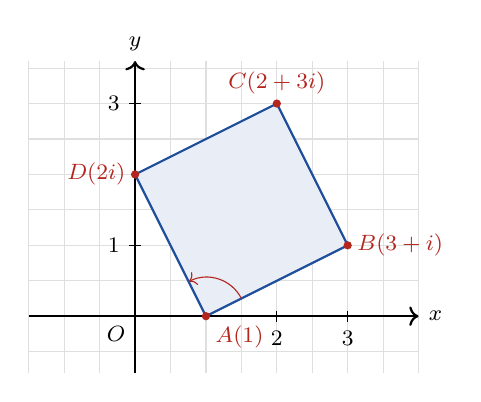
\begin{tikzpicture}[x=0.9cm,y=0.9cm,font=\footnotesize]\draw[gray!25,step=0.5] (-1.5,-0.8) grid (4,3.6);\draw[->,thick] (-1.5,0)--(4,0) node[right]{$x$}; \draw[->,thick] (0,-0.8)--(0,3.6) node[above]{$y$};\draw (2,0.08)--(2,-0.08) node[below]{$2$};\draw (3,0.08)--(3,-0.08) node[below]{$3$};\draw (0.08,1)--(-0.08,1) node[left]{$1$};\draw (0.08,3)--(-0.08,3) node[left]{$3$};\node[below left] at (0,0){$O$};\draw[cDef,thick,fill=cDef!10] (1,0)--(3,1)--(2,3)--(0,2)--cycle;
\fill[cThm] (1,0) circle (1.5pt) node[below right]{$A(1)$}; \fill[cThm] (3,1) circle (1.5pt) node[right]{$B(3+i)$};
\fill[cThm] (2,3) circle (1.5pt) node[above]{$C(2+3i)$}; \fill[cThm] (0,2) circle (1.5pt) node[left]{$D(2i)$};
\draw[cThm,->] (1.5,0.25) arc (27:117:0.55);\end{tikzpicture}\end{LTR}\par }{}{}
\Row{بناء المعارف}{%
\Lab{cMeth}{طريقة}\par\textbf{(1)} نترجم الوضعية الهندسية إلى تحويل (دوران ، تحاكٍ ، انسحاب).\par\textbf{(2)} نكتب كتابته المركبة ، ثم نحسب اللواحق.}{50 د}{رسم الشكل.}
\Row{}{%
\Lab{cEx}{أمثلة محلولة}\par\textbf{(1)} مثلث متقايس الأضلاع مباشر $ABC$ مع $A(0)$ ، $B(2)$: \par $z_C=e^{i\frac\pi3}z_B=2\left(\dfrac12+i\dfrac{\sqrt3}2\right)=\RR{1+i\sqrt3}$.\par\textbf{(2)} صورة $M(2+i)$ بالتحاكي الذي مركزه $O$ ونسبته $3$: $\RR{6+3i}$.}{}{}
\Row{}{%
\Lab{cThm!80!black}{حذار}\ نراعي الاتجاه: مباشر (زاوية $+\frac\pi2$) أو غير مباشر ($-\frac\pi2$).}{}{}
\Row{التقويم}{%
\Lab{cMeth}{تمرين تطبيقي}\par $A(i)$ ، $B(2+i)$.\par\textbf{(1)} عيّن لاحقة $C$ حيث $ABC$ قائم ومتساوي الساقين في $A$ ومباشر.}{25 د}{تقويم فردي.}
\Row{}{%
\Lab{cEx}{حل التمرين التطبيقي}\par\textbf{(1)} $z_C=z_A+i(z_B-z_A)=i+i\times2=\RR{3i}$.\par\textbf{واجب منزلي:} تمارين من باب الأعداد المركبة.\par\smallskip\textbf{ملاحظات حول سير الحصة:} \dotfill}{}{}
\end{Sayr}
\newpage
\ModhHead{76}{3 ع ت / 3 ر / 3 ت ر}{أعداد وحساب}{الأعداد المركبة والتحويلات النقطية}{02 سا}{التشابه المباشر: تعريف ، كتابته المركبة ، عناصره}%
{\begin{itemize}\item التحويلات المألوفة وكتاباتها المركبة.\end{itemize}}%
{\begin{itemize}\item التعرف على التشابه المباشر وتعيين عناصره المميزة.\end{itemize}}%
{المنهاج ، الكتاب المدرسي (الجزء الثاني) ، الآلة الحاسبة ، أدوات الهندسة.}
\begin{Sayr}
\Row{مرحلة الانطلاق}{%
\textbf{التهيئة النفسية:} ما التحويل الذي يكبّر ويدير في آن واحد؟}{10 د}{سؤال.}
\Row{التشخيص والاكتشاف}{%
\Lab{cEx}{نشاط رقم 10}\ $z^{\prime}=(1+i)z$.\par\textbf{(1)} قارن $|z^{\prime}|$ بـ $|z|$ ، و $\arg z^{\prime}$ بـ $\arg z$.\par\textbf{(2)} صف التحويل.}{35 د}{مثال بالضرب.}
\Row{}{%
\Lab{cDef}{مناقشة النشاط}\par\textbf{(1)} $|z^{\prime}|=\sqrt2|z|$ ؛ \quad $\arg z^{\prime}=\arg z+\dfrac\pi4$.\par\textbf{(2)} تكبير بالنسبة $\sqrt2$ ودوران بـ $\dfrac\pi4$ حول $O$: \RR{تشابه} \RR{مباشر}.}{}{}
\Row{بناء المعارف}{%
\Lab{cDef}{تعريف}\ \textbf{التشابه المباشر} تحويل كتابته المركبة $\LW{\RR{z^{\prime}=az+b}}$ مع $\LW{a\in\mathbb C^*}$.}{50 د}{جدول العناصر.}
\Row{}{%
\Lab{cThm}{العناصر المميزة ($a
eq1$)}\par\textbf{(1)} النسبة $\LW{\RR{k=|a|}}$ ، الزاوية $\LW{\RR{\theta=\arg a}}$ ، المركز $\LW{\RR{\omega=\dfrac b{1-a}}}$.\par\textbf{(2)} الانسحابات والدورانات والتحاكيات حالات خاصة ، والتشابه الذي نسبته $\LW{1}$ \textbf{تقايس}.}{}{}
\Row{}{%
\Lab{cEx}{أمثلة محلولة}\par\textbf{(1)} $z^{\prime}=(1+i)z+2$: $k=\RR{\sqrt2}$ ، $\theta=\RR{\dfrac\pi4}$ ، $\omega=\dfrac2{-i}=\RR{2i}$.\par\textbf{(2)} $z^{\prime}=-3iz$: $k=\RR{3}$ ، $\theta=\RR{-\dfrac\pi2}$ ، المركز $\RR{O}$.}{}{}
\Row{}{%
\Lab{cThm!80!black}{حذار}\ إذا كان $a=1$ فهو انسحاب (لا مركز له).}{}{}
\Row{التقويم}{%
\Lab{cMeth}{تمرين تطبيقي}\par\textbf{(1)} عيّن عناصر التشابه $z^{\prime}=(1+i\sqrt3)z-i\sqrt3$.}{25 د}{تقويم فردي.}
\Row{}{%
\Lab{cEx}{حل التمرين التطبيقي}\par\textbf{(1)} $k=|1+i\sqrt3|=\RR{2}$ ؛ \quad $\theta=\RR{\dfrac\pi3}$.\par\textbf{(2)} $\omega=\dfrac{-i\sqrt3}{1-1-i\sqrt3}=\RR{1}$.\par\textbf{واجب منزلي:} تمارين من باب التشابهات.\par\smallskip\textbf{ملاحظات حول سير الحصة:} \dotfill}{}{}
\end{Sayr}
\newpage
\ModhHead{77}{3 ع ت / 3 ر / 3 ت ر}{أعداد وحساب}{الأعداد المركبة والتحويلات النقطية}{02 سا}{التحليل القانوني لتشابه مباشر ، مركب تشابهين}%
{\begin{itemize}\item التشابه المباشر وعناصره.\end{itemize}}%
{\begin{itemize}\item تعيين التحليل القانوني لتشابه مباشر ، وتعيين مركب تشابهين.\end{itemize}}%
{المنهاج ، الكتاب المدرسي (الجزء الثاني) ، الآلة الحاسبة ، أدوات الهندسة.}
\begin{Sayr}
\Row{مرحلة الانطلاق}{%
\textbf{التهيئة النفسية:} هل يمكن كتابة تشابه كتركيب تحويلين أبسط؟}{10 د}{سؤال.}
\Row{التشخيص والاكتشاف}{%
\Lab{cEx}{نشاط رقم 11}\ $s$: \par $z^{\prime}-\omega=ke^{i\theta}(z-\omega)$.\par\textbf{(1)} $r$: $z_1-\omega=e^{i\theta}(z-\omega)$ و $h$: $z^{\prime}-\omega=k(z_1-\omega)$. احسب $h\circ r$.\par\textbf{(2)} هل $r\circ h=h\circ r$ ؟}{35 د}{التحليل.}
\Row{}{%
\Lab{cDef}{مناقشة النشاط}\par\textbf{(1)} $z^{\prime}-\omega=k\,e^{i\theta}(z-\omega)$: $\RR{h\circ r=s}$.\par\textbf{(2)} $ke^{i\theta}=e^{i\theta}k$: \RR{نعم} ، الترتيب لا يهم لأن لهما نفس المركز.}{}{}
\Row{بناء المعارف}{%
\Lab{cThm}{التحليل القانوني}\ التشابه $\LW{s}$ الذي مركزه $\LW{\Omega}$ ونسبته $\LW{k}$ وزاويته $\LW{\theta}$: $\LW{\RR{s=h\circ r=r\circ h}}$ حيث $\LW{h}$ التحاكي $\LW{(\Omega;k)}$ و $\LW{r}$ الدوران $\LW{(\Omega;\theta)}$.}{50 د}{جدول المركب.}
\Row{}{%
\Lab{cThm}{مركب تشابهين}\ مركب تشابهين مباشرين تشابه مباشر: \RR{النسبة} \RR{جداء} \RR{النسبتين} و\RR{الزاوية} \RR{مجموع} \RR{الزاويتين}.}{}{}
\Row{}{%
\Lab{cEx}{أمثلة محلولة}\par\textbf{(1)} $s_1$: $z^{\prime}=2z+1$ ، $s_2$: $z^{\prime}=iz$: $s_2\circ s_1$: $z^{\prime\prime}=i(2z+1)=\RR{2iz+i}$.\par\textbf{(2)} نسبته $\RR{2}$ ، زاويته $\RR{\dfrac\pi2}$ ، مركزه $\omega=\dfrac i{1-2i}=\RR{\dfrac{-2+i}5}$.}{}{}
\Row{}{%
\Lab{cThm!80!black}{حذار}\ عمومًا $s_2\circ s_1\neq s_1\circ s_2$: $s_1\circ s_2$: $z^{\prime\prime}=2iz+1$.}{}{}
\Row{التقويم}{%
\Lab{cMeth}{تمرين تطبيقي}\par\textbf{(1)} $s$: $z^{\prime}=(1+i)z$. عيّن $s\circ s$ وعناصره.}{25 د}{تقويم فردي.}
\Row{}{%
\Lab{cEx}{حل التمرين التطبيقي}\par\textbf{(1)} $z^{\prime\prime}=(1+i)^2z=\RR{2iz}$: نسبته $\RR{2}$ ، زاويته $\RR{\dfrac\pi2}$ ، مركزه $\RR{O}$.\par\textbf{واجب منزلي:} تمارين من باب التشابهات.\par\smallskip\textbf{ملاحظات حول سير الحصة:} \dotfill}{}{}
\end{Sayr}
\newpage
\ModhHead{78}{3 ع ت / 3 ر / 3 ت ر}{أعداد وحساب}{الأعداد المركبة والتحويلات النقطية}{02 سا}{خواص التشابه المباشر وحل مسائل}%
{\begin{itemize}\item التشابه المباشر ، التحليل القانوني.\end{itemize}}%
{\begin{itemize}\item توظيف خواص التشابه لحل مسائل هندسية ، وتعيين تشابه يحول نقطتين إلى نقطتين.\end{itemize}}%
{المنهاج ، الكتاب المدرسي (الجزء الثاني) ، الآلة الحاسبة ، أدوات الهندسة.}
\begin{Sayr}
\Row{مرحلة الانطلاق}{%
\textbf{التهيئة النفسية:} كم تشابهًا مباشرًا يحول $A$ إلى $A^{\prime}$ و $B$ إلى $B^{\prime}$ ؟}{10 د}{سؤال.}
\Row{التشخيص والاكتشاف}{%
\Lab{cEx}{نشاط رقم 12}\ $A(0)\mapsto A^{\prime}(1)$ ، $B(1)\mapsto B^{\prime}(1+i)$.\par\textbf{(1)} اكتب الجملة التي يحققها $a$ و $b$ في $z^{\prime}=az+b$.\par\textbf{(2)} حلها وعيّن عناصر التشابه.}{35 د}{جملة معادلتين.}
\Row{}{%
\Lab{cDef}{مناقشة النشاط}\par\textbf{(1)} $b=1$ و $a+b=1+i$.\par\textbf{(2)} $\RR{a=i}$ ، $\RR{b=1}$: $z^{\prime}=iz+1$: دوران زاويته $\dfrac\pi2$ ومركزه $\omega=\dfrac1{1-i}=\RR{\dfrac{1+i}2}$.}{}{}
\Row{بناء المعارف}{%
\Lab{cThm}{خاصية}\par\textbf{(1)} التشابه المباشر يحافظ على \RR{نسب} \RR{المسافات} \RR{والزوايا} \RR{الموجهة} والاستقامية والتوازي.\par\textbf{(2)} من أجل $\LW{A\neq B}$ و $\LW{A^{\prime}\neq B^{\prime}}$ يوجد تشابه مباشر وحيد: \par $\LW{\RR{a=\dfrac{z_{B^{\prime}}-z_{A^{\prime}}}{z_B-z_A}}}$ ، $\LW{\RR{b=z_{A^{\prime}}-az_A}}$.\par\textbf{(3)} صورة دائرة مركزها $\LW{\Omega}$ ونصف قطرها $\LW{R}$: دائرة مركزها $\LW{s(\Omega)}$ ونصف قطرها $\LW{kR}$.}{50 د}{رسم الصور.}
\Row{}{%
\Lab{cEx}{مثال محلول}\ $s$: $z^{\prime}=2iz-i$ ، والدائرة $(\mathcal C)$: مركزها $\Omega(1)$ ونصف قطرها $1$.\par\textbf{(1)} $s(\Omega)$: $2i\times1-i=\RR{i}$ ؛ \quad $k=|2i|=2$.\par\textbf{(2)} صورة $(\mathcal C)$: \RR{دائرة} \RR{مركزها} \RR{$(0;1)$} \RR{ونصف} \RR{قطرها} \RR{$2$}.}{}{}
\Row{}{%
\Lab{cThm!80!black}{حذار}\ صورة دائرة دائرة: نحول المركز ونضرب نصف القطر في $k$.}{}{}
\Row{التقويم}{%
\Lab{cMeth}{تمرين تطبيقي}\par\textbf{(1)} عيّن التشابه الذي يحول $A(1)$ إلى $A^{\prime}(i)$ و $B(2)$ إلى $B^{\prime}(3i)$.\par\textbf{(2)} عيّن عناصره.}{25 د}{نهاية المحور: فرض أو مراجعة.}
\Row{}{%
\Lab{cEx}{حل التمرين التطبيقي}\par\textbf{(1)} $a=\dfrac{3i-i}{2-1}=\RR{2i}$ ؛ \quad $b=i-2i\times1=\RR{-i}$: $z^{\prime}=2iz-i$.\par\textbf{(2)} $k=\RR{2}$ ، $\theta=\RR{\dfrac\pi2}$ ، $\omega=\dfrac{-i}{1-2i}=\RR{\dfrac{2-i}5}$.\par\textbf{واجب منزلي:} مسائل من باب التشابهات.\par\smallskip\textbf{ملاحظات حول سير الحصة:} \dotfill}{}{}
\end{Sayr}
\end{document}
